\section[Выбор и обоснование средств реализации]{ВЫБОР И ОБОСНОВАНИЕ \\ СРЕДСТВ РЕАЛИЗАЦИИ}
\label{sec:choice}

\subsection{Выбор операционной системы}

До начала стадии проектирования приложения необходимо решить,
для какой операционной системы оно будет разрабатываться.
Среди кандитов выступают следующие операционные системы:
\begin{itemize}
  \item Windows 8.1;
  \item дистрибутив Linux (Elementary OS);
  \item OS X 10.10.
\end{itemize}

Рассмотрим каждую из приведенных операционных систем подробнее.

В ходе специального мероприятия Build 2013 компания Microsoft представила
предварительную версию первого крупного обновления для Windows --- Windows 8.1.
Большинство изменений в Windows 8.1 заметны уже со стартового экрана --- они
касаются в основном фирменного пользовательского интерфейса Metro. Теперь
пользователю доступна более тонкая настройка <<плиток>> на главном экране,
улучшена поддержка жестов, кнопка <<Пуск>> вернулась на привычное для неё место.

По сравнению с предшественниками, Windows 8.1 стала более легковесной,
в несколько раз был ускорен режим <<сна>>, встроенный интернет-браузер IE
стал гораздо быстрее работать.

С точки зрения разработчиков появилась возможность попробывать себя в создании
приложений для <<плиточного>> интерфейса от Microsoft, который лучше всего
проявляет себя на ноутбуках и планшетных компьютерах с сенсорным экраном.

Высокая доля использования системы от Microsoft среди пользователей делает её
самой обсуждаемой ОС на всевозможных технических форумах. Таким образом,
задавшись каким-либо вопросом, есть большая вероятность отыскать ответ на
аналогичный вопрос с помощью интернет-поисковиков. Если же ответ не будет
найден, можно задать свой вопрос на специализированных форумах и ответ не
заставит себя долго ждать.

Производить мониторинг потока событий в операционной системе Windows 8.1
лучше всего с помощью инструментария WMI, который обсуждался
в подразделе~\ref{sub:monitoring_tools}. Использование WMI для обработки
событий в Windows имеет свои достоинства и недостатки. Приведём достоинства
использования WMI:
\begin{itemize}
  \item унифицированный интерфейс для управления системами Windows;
  \item свобода в выборе языка программирования;
  \item широкий охват <<узлов>> операционной системы.
\end{itemize}

К недостаткам можно отнести следующие особенности инструментария управления
Windows:
\begin{itemize}
  \item огромное число классов, в которых легко запутаться;
  \item специфический синтаксис построения запросов;
  \item низкая скорость работы некоторых запросов.
\end{itemize}

Одной из главных особенностей операционной системы Linux является наличие
бесплатных дистрибутивов, таких как Ubuntu, Fedora, Gentoo, Elementary OS и другие.
Это может существенно сократить расходы как обычному пользователю,
так и большим предприятиям, которым необходимо установить операционную
систему на несколько сотен, а то и тысяч компьютеров.

Отдельно стоит упомянуть гибкость дистрибутивов Linux --- практически из
любого компьютера можно сделать полноценный сервер. Это делает дистрибутивы
Linux очень привлекательными для программистов, которым приходится сталкиваться
с веб-программированием.  Пользователь получает
возможность запускать только те процессы, которые интересны именно ему, а не те,
которые по умолчанию установлены системой.

Благодаря открытому сообществу разработчиков, в дистрибутивах Linux можно
встретить массу современных веяний в сфере операционных систем: оформления
окон, оригинальное использование панели задач, боковых панелей и так далее.

Большинство дистрибутивов Linux поставляются с широким предустановленным
пакетом программ, таким образом пользователь избавляет себя от траты времени
и денег на установку дополнительных программных продуктов. В том случае, если
пользователь не обнаружил необходимую программу среди предустановленных, он
может воспользоваться пакетным менеджером, предоставляющим доступ к
множеству доступных для скачивания программ в соответствующих репозиториях.

Дистрибутив Elementary OS, как и множество дистрибутивов системы Linux,
распространяется бесплатно. Основными достоинствами данного дистрибутива,
кроме свободной лицензии, является простота в использовании,
интуитивно понятный интерфейс, и внешняя схожесть с последними версиями
операционной системы от Apple.
% elementaryos.org

Интерфейс дистрибутива Elementary OS представлен на рисунке~\ref{pic:elementary}.
\begin{figure}[h!]
  \centering
  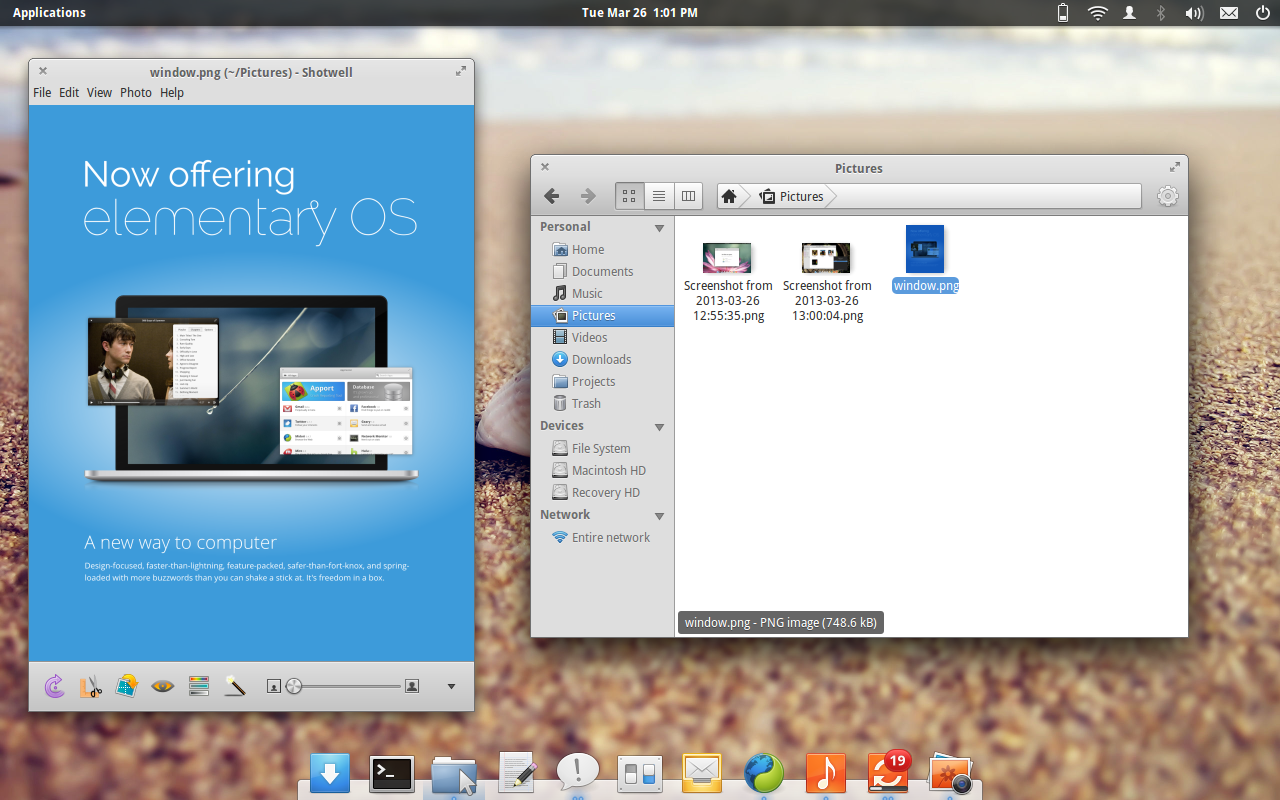
\includegraphics[width=150mm]{pic/elementary.png}
  \caption{Интерфейс дистрибутива Elementary OS}
  \label{pic:elementary}
\end{figure}

OS X --- операционная система, лежащая в основе каждого Mac. Она построена на
базе надежной платформы UNIX и задействует все возможности аппаратного обеспечения.
Её простота и удобство не уступает красоте её интерфейса. В состав OS X входит
отличная коллекция приложений на каждый день. И она даёт замечательные возможности
для совместной работы компьютера Mac и мобильных устройств под управлением iOS.
%https://www.apple.com/ru/osx/what-is/

Операционная система от Apple является симбиозом надёжности, производительности
и великолепного интерфейса. Отдельного внимания заслуживают поставляемые с
операционной системой программы, такие как Calendar, Safari, iPhoto и другие.
Все они готовы к безупречной работе сразу после установки OS X на компьютер Mac.

Ещё одной сильной стороной операционной системы от Apple является язык Objective-C,
который используется для создания приложений для OS X и для мобильных устройств.
ObjC был создан Брэдом Коксом в начале 1980-х годов в его компании Stepstone.
Он пытался решить проблему повторного использования кода.
Целью Кокса было создание языка, поддерживающего концепцию software IC.
Под этой концепцией понимается возможность собирать программы
из готовых компонентов (объектов), подобно тому как сложные электронные устройства
могут быть легко собраны из набора готовых интегральных микросхем.

При этом такой язык должен был быть достаточно простым и основанным на языке С,
чтобы облегчить переход разработчиков на него. Одной из целей было также
создание модели, в которой сами классы также являются полноценными объектами,
поддерживалась бы интроспекция и динамическая обработка сообщений.

Получившийся в результате язык Objective-C оказался крайне прост~---~его освоение
у С-программиста займет всего несколько дней. Он является именно расширением
языка С --- в язык С просто добавлены новые возможности для
объектно-ориентированного программирования. При этом любая программа на С
является программой и на Objective-C.

Одной из отличительных черт Objective-C является его динамичность~---~целый ряд
решений, обычно принимаемых на этапе компиляции, здесь откладывается
непосредственно до этапа выполнения.

Возможности по обработке потока событий с использованием языка Objective-C
были рассмотрены в подразделе~\ref{sub:monitoring_tools}.


\subsection{Выбор среды разработки}

Стандартом в разработке приложений на Objective-C до недавних пор была
среда разработки от Apple --- Xcode. Но в апреле 2011 года компания JetBrains
представила AppCode. Рассмотрим каждую из приведенных сред разработки подробнее.

Xcode --- самодостаточная среда разработки программного обеспечения от Apple,
включающая в себя полноценный текстовый редактор, большую часть документации
от Apple и Interface Builder. IB~---~приложение, использующееся для создания
графических приложений. Скачивая инструментарий разработчика Xcode,
пользователь также получает программу iOS Simulator, позволяющую тестировать
создаваемые приложения для мобильных устройств на компьютере Mac.
Актуальная версия интегрированной среды от Apple --- Xcode 6.1.1
появилась в Mac App Store 2 декабря 2014 года.
%apple xcode

Среда разработки Xcode 6.1.1 обладает следующими достоинствами:
\begin{itemize}
  \item распространяется бесплатно через Mac App Store;
  \item практически тотальное использование у Objective-C разработчиков;
  \item принцип <<всё включено>>: встроена документация, программа для
    разработки интерфейса и так далее.
\end{itemize}

Недостатки интегрированной среды разработки от Apple:
\begin{itemize}
  \item низкая скорость реакции на веяния рынка, зависящая от взглядов Apple
    на эти веяния;
  \item недостаточная кастомизация интерфейса.
\end{itemize}

AppCode --- альтернатива для разработчиков на языке Objective-C, предложенная
компанией JetBrains. Интегрированная среда построена на основе флагмана
компании --- IntelliJ IDEA.
%jetbrains appcode

Можно выделить следующие достоинства AppCode:

\begin{itemize}
  \item продуманная система рефакторинга;
  \item темный вариант оформления интерфейса;
  \item интеграция с issue-треккерами, такими как JIRA, YouTrack и другими.
\end{itemize}

К недостаткам AppCode можно отнести косвенную зависимость от
IDE Xcode~(необходимость поддержки полной совместимости), а также распространение
на платной основе.

Учитывая приведенные достоинства и недостатки рассматриваемых в этом разделе
систем, выбор был сделан в пользу операционной системы OS X, языка программирования
Objective-C и интегрированной среды разработки Xcode.

\pagebreak
